\documentclass{beamer}
\usepackage{geometry}
\usepackage[english]{babel}
\usepackage[utf8]{inputenc}
\usepackage{amsmath}
\usepackage{amsfonts}
\usepackage{amssymb}
\usepackage{tikz}
\usepackage{graphicx}
\usepackage{venndiagram}

%\usepackage{pgfplots}
%\pgfplotsset{width=10cm,compat=1.9}
%\usepackage{pgfplotstable}

\setlength{\headheight}{26pt}%doesn't seem to fix warning

\usepackage{fancyhdr}
\pagestyle{fancy}
\fancyhf{}

%\rhead{\small{23 April 2018}}
\lhead{\small{BECA / Dr. Huson / Mathematics}}

%\vspace{1cm}

\renewcommand{\headrulewidth}{0pt}


\title{Mathematics Class Slides}
\subtitle{Bronx Early College Academy}
\author{Chris Huson}
\date{3 May 2018}

\begin{document}

\frame{\titlepage}

%\section[Outline]{}
%\frame{\tableofcontents}

\section{11.2 Algebra II Drui}
\frame
{
  \frametitle{How do we convert the base of an exponential function?}
  \framesubtitle{CCSS: HSF.LB.B.5 Interpret the parameters in an exponential function \qquad \alert{11.2}}

  \begin{block}{Do Now: Interest calculations, assume principal is \$100.}
  \begin{enumerate}
      \item Calculate interest for 6 months with an annual rate of 5\%.
      \item After one year at an annual rate of 5.25\%, what would be the combined principal and interest?
      \item How many interest payments would there be in two years given monthly compounding?
      \item If the interest after one month is \$1.50, what would the annual interest rate be? 
  \end{enumerate}
  \end{block}
  Lesson: Continuously compounded interest\\*
  Task: Practice problems\\*
  Assessment: Convert to an annual rate given $P=P_0e^{0.05x}$\\*
  Homework: Exponential function \& review problems\\
}


\section{12.1 IB Math SL Drui}
\frame
{
  \frametitle{GQ: How do we prepare for the IB final exams?}
  \framesubtitle{CCSS: HSF.IF.B.4 Interpret key features of functions and their graphs \qquad \alert{12.1}}

  \begin{block}{Do Now: 1st \& 2nd derivatives of a cubic function, sketch}
    \begin{enumerate}
    \item Given the function $f(x)=x^3-9x$
    \item Find $f'(x)$ and $f''(x)$.
    \item Sketch $f$ and its two derivatives on the same set of axes. Label the intersections and extrema.
    \end{enumerate}
 \end{block}
  Lesson: Last minute study practices (reflection) \\[5pt]
  Task: Homework review: Work homework problems on board\\%*[5pt]
  Assessment: Problem set and exam mark scheme\\%*[5pt]
  Homework: Prepare for final exams
}

\section{11.1 IB Math SL Drui}
\frame
{
  \frametitle{How do we compare two variables?}
  \framesubtitle{CCSS: HSS.IC.A.1 Understand statistics as a process for making inferences about a population \qquad \alert{11.1}}

  \begin{block}{Do Now: Given two independent events with probability 0.6 and 0.5. }
  \begin{enumerate}
      \item What is the probability of both happening together? 
      \item Draw a Venn diagram representing their intersection.
  \end{enumerate}
  \end{block}
  Lesson: Applying independence tests in a real world context. Picking an exploration topic\\*
  Task: Regression of bivariate data. Exercise 10A \#4 p 339\\*
  Assessment: Test corrections due today\\*
  Homework: Statistics textbook problems 10B p. 341\\
}

\frame
{
  \frametitle{Steps for writing technical papers}
  \framesubtitle{Practice writing mathematics according to IB requirements, as per IA criteria.}
Proposal
\begin{enumerate}
    \item Define an ``aim," including success criteria. 
    \item Outline paper, especially Method including data collection, graphs, formulas; list references
    \item Draft introduction, including rationale and aim.
    \item Structure data tables, sketch graphs, begin formula and algebra (all handwritten, perhaps spreadsheets or Desmos)
    \item Draft Method section text
\end{enumerate}
Method
\begin{enumerate}
    \item Collect data (survey, search, simulation, etc.)
    \item Work interactively with spreadsheets, graphing software, math
    \item Refine Method section, draft results and discussion.
\end{enumerate}
Complete mathematics and paper. Proofread carefully. Rewrite. Receive peer feedback. Rewrite. Submit final draft.
}


\frame
{
  \frametitle{Standards for writing technical papers}
  \framesubtitle{Practice writing mathematics according to IB requirements, as per IA criteria.}
Criterion C: Personal engagement (0-4 points)
\begin{enumerate}
    \item Address a personal interest; ``make it your own"
    \item Think independently and/or creatively
    \item Present mathematical ideas in your own way 
\end{enumerate}
Criterion D: Reflection (0-3 points)
\begin{enumerate}
    \item Review, analyze, and evaluate the mathematics throughout the paper. Go beyond just describing results
    \item Link to the aims, comment on what has been learned, consider limitations, and compare different mathematical approaches
    \item Consider what's next, discuss the implications of results, strengths and weaknesses of approaches, and consider different perspectives
\end{enumerate}
}


\frame
{
  \frametitle{Standard conventions for mathematical notation}
  \framesubtitle{Practice writing mathematics according to IB requirements, as per exam rubrics.}
\begin{enumerate}
    \item Use the formula sheet.
    \item Chose the appropriate formula (M1).\\*
    (you do not have to copy the formula)
    \item Substitute values correctly (A1). 
    \item Solve, showing key steps (A1).\\
    (skip routine algebra if you like)
    \item Write down the exact solution or copy the calculator display. An ellipsis (\ldots) indicates more digits (A1).
    \item Round to 3 significant digits (use $\approx$)(A1).
\end{enumerate}
}

\frame
{
  \frametitle{Standard conventions for mathematical notation}
  \framesubtitle{Practice writing mathematics according to IB requirements, as per exam rubrics.}
Examples of key algebraic techniques
\begin{enumerate}
    \item Setting a quadratic function $=0$
    \item Converting an exponent to a log
    \item Reading a value from a graph
    \item When writing lists, you may write only the first two and the last terms. For example,
\[\sum_{k=1}^5 3 \cdot 2.25^k =3 + 6.75+\ldots+76.8867\ldots\]
\[=135.99609\ldots \approx 136\]
\end{enumerate}
}


\frame
{
  \frametitle{Descriptive statistics terminology}
  \framesubtitle{Make a list of these terms, find their definitions in the textbook.}
  
  Univariate data, bivariate\\*
  Population, sample, random/biased sample, survey, census\\*
  Discrete/continuous data, quantitative/qualitative\\* 
  Central tendency, mean ($\overline{x}, \mu$), median, mode; quartiles, percentiles\\*
  5-figure summary, box \& whisker plots, range, interquartile range, outlier\\*
  Dispersion, standard deviation ($\sigma$), variance ($v=\sigma^2$)\\*
  Frequency distributions (tables/bar charts/histograms)\\*
  Grouped data, class, mid-interval value, boundaries, modal class\\*
  Cumulative frequency distributions

  
}

\frame
{
  \frametitle{Bias and fairness, random variation, \& combinations}
  \framesubtitle{When rolling two dice, why aren't all the possible totals equally likely?}
  Definition:\\*
  A \alert{fair} (p. 67) or \alert{unbiased} (p. 79) process \\*[15pt]
  In mathematics we usually simplify and assume a random process follows exact, idealized probabilities. For example, we assume heads and tails are equally likely results of a coin toss.
  
}

\frame
{
  \frametitle{Bias and fairness, random variation, \& combinations}
  \framesubtitle{When rolling two dice, why aren't all the possible totals equally likely?}
  Definition:\\*
  \alert{Experimental} or \alert{empirical} (p. 65) results \\*[15pt]
  In real life, the results of any experiment have a degree of \alert{random variation}. The observed relative frequencies are estimates of the underlying theoretical probabilities, which grow more accurate with additional trials.
  
}

\frame
{
  \frametitle{Bias and fairness, random variation, \& combinations}
  \framesubtitle{When rolling two dice, why aren't all the possible totals equally likely?}
  Counting events in a \alert{sample space} (p. 78) or calculating \alert{combinations} (p. 184) \\*[15pt]
  The six possible results of rolling a single die are equally likely, $\mathrm P(x)=\frac{1}{6}$, if we assume the die is fair. Similarly, the probability of any of the 36 $(6 \times 6)$ possible results of rolling two dice are equally likely, $\mathrm P(x)=(\frac{1}{6})^2$. However, the probability of a particular total varies according to how many combinations lead to that total. Thus, for example, 7 can be rolled six different ways, so $\mathrm P(7)=\frac{6}{36}$, while 2 can only result one way, $\mathrm P(2)=\frac{1}{36}$.
  
}

\frame
{
  \frametitle{Sets, subsets, \& proper subsets}
  
  Definitions:\\*
  A \alert{set} is an unordered collection of elements.\\ e.g. \{red, white, blue\} (do not repeat elements)\\*[5pt]
  \alert{Subset}: Set $A$ is a subset of set $B$ if and only if all of the elements of $A$ are elements of $B$.\\
  Written: $A \subseteq B$\\[5pt]
  \alert{Proper subset}: $A \subseteq B$ and $A$ is not equal to $B$. Written: $A \subset B$\\[5pt]
  The \alert{empty set} is a subset of all sets. $\{\} \text{ or } \emptyset$
  
}


\frame
{
  \frametitle{The volume of a function rotated around the $x$-axis}
  \framesubtitle{Differentiate over $x$, but use the area of a disk defined by $A=\pi r^2$}
\href{https://www.youtube.com/watch?v=i4L5XoUBD_Q}{video}\\
\begin{figure}[!ht]
    \centering
    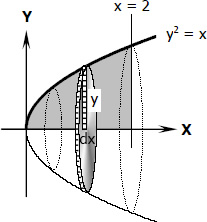
\includegraphics[width=0.5\textwidth]{0413CW-paraboloid.jpg}
\end{figure}
\small{Credit: MATHalino.com - Pinoy Math Community Romel Verterra}
}

\frame
{
  \frametitle{GQ: Combinatorics problem}
  \framesubtitle{CCSS: F.IF.B.6 Calculate \& interpret the rate of change of a function}

  \begin{block}{Show the formula and then use your calculator function}
  \begin{enumerate}
      \item You have a \$1 bill, a \$5 bill, a \$10 bill, a \$20 bill, a quarter, a dime, a nickel, and a penny. How many different total amounts can you make by choosing six bills and coins?
  \end{enumerate}
  \end{block}
  What is the number of the set you are choosing from?\\%*[5pt]
  How many are you picking?\\%*[5pt]
  Does their order matter?
}

\begin{frame}{Do Now \#1: Phone preferences by gender}
    \framesubtitle{Given the frequency table, make a Venn diagram}
    \begin{tabular}{l|c|r|}
        & Android & iPhone\\ 
        \hline 
        Boys & 15 & 5 \\ 
        \hline 
        Girls & 5 & 15 \\
        \hline 
    \end{tabular}\\*[10pt]
    \centering
    $A=\{ \text{prefers Android}\}$ and $B=\{ \text{is a boy}\}$
    \begin{venndiagram2sets}[tikzoptions={scale=1.0}]
    \end{venndiagram2sets}
\end{frame}

\begin{frame}{Do Now \#2: Independence}
    \framesubtitle{Given the situation, make a Venn diagram, frequency table, and tree representing}
    $\mathrm{P}(A)=0.6$, $\mathrm{P}(B)=0.5$, $\mathrm{P}(A \cap B)=0.3$
    \centering
    \begin{venndiagram2sets}[tikzoptions={scale=1.0}]
    \end{venndiagram2sets}\\*[10pt]
    \begin{tabular}{l|c|r|}
        & $A$ & $A^\prime$\\ 
        \hline 
        $B$ &  \qquad \qquad &  \qquad \qquad \\ 
        \hline 
        $B^\prime$ &  &  \\
        \hline 
    \end{tabular}\\*[10pt]
\end{frame}

\begin{frame}{$\mathrm P(A \cup B) = \mathrm P(A) + \mathrm P(B) - \mathrm P(A \cap B)$}
    \framesubtitle{The addition rule}
    \begin{venndiagram2sets}[tikzoptions={scale=2}]
    \end{venndiagram2sets}
\end{frame}

\begin{frame}{Distributions}
    \framesubtitle{Tables and charts used to summarize a problem situation}
    A \alert{frequency distribution} displays the number of times each event in the sample space occurs, either in tabular or graphical form.\\*[10pt]
    A \alert{probability distribution} shows the same data, normalizing the totals to one.
\end{frame}


\begin{frame}{Technical writing}
    \framesubtitle{Write a short paper answering the query: \\* "How many subsets can be picked from a group of four students?"}
    \begin{enumerate}
        \item Logical, step-by-step explanation, using an example
        \item Precise terminology, succinct: combination, permutation, order (matters), event, sample space, set, subset, with /without replacement, factorial
        \item Notation: algebra symbols, tables, trees, grids
        \item Summary, big-picture, conceptual idea
        \item Audience: student peers
    \end{enumerate}
\end{frame}





\begin{frame}{Combinatorics formulas}
    \alert{Combinations}, when order doesn't matter
	$$_nC_r = \frac{n!}{(n-r)! r!} \qquad \text{''n pick r"}$$
    \alert{Permutations}, when order does matter
	$$_nP_r = \frac{n!}{(n-r)!} $$
\end{frame}

\begin{frame}{Definition of theoretical probability}
    The \alert{theoretical probability} of an event $A$ is $\displaystyle \mathrm P(A) = \frac{n(A)}{n(U)}$\\*[10pt]
    \quad where $n(A)$ is the number of ways an event can occur\\*[5pt]
    \quad and $n(U)$ is the total number of possible outcomes (p. 65)\\*[10pt]
    Theoretically, in $n$ trials, one would expect the event to occur $n \times \mathrm P(A)$ times\\*[10pt]
    Probabilities are between 0 and 1, inclusive. $0 \leq \mathrm P(X) \leq 1$
\end{frame}

\begin{frame}{Empirical (experimental) probability}
    The \alert{relative frequency} of an event can be used as an estimate of its probability. $$\displaystyle \mathrm P(A) = \frac{\text{number of occurrences of event } A}{\text{total number of trials}}$$
    The larger the number of trials the more reliable the estimate of probability.
\end{frame}

\begin{frame}{Independence and mutual exclusivity}
    Two events are \alert{independent} if the occurrence of one does not affect the probability of the other. $$\displaystyle \mathrm P(\text{both }A \text{ and }B \text{ occur}) = \mathrm P(A) \times \mathrm P(B)$$
    Two events are \alert{mutually exclusive} if they never occur together. 
    $$\displaystyle \mathrm P(\text{both }A \text{ and }B \text{ occur}) = 0 \qquad \text{and}$$
    $$\mathrm P(\text{either }A \text{ or }B \text{ occur}) = \mathrm P(A) + \mathrm P(B)$$
\end{frame}

\begin{frame}{Venn diagrams}
    \framesubtitle{For organizing compound events}
    When two events can occur, and perhaps both, or neither.
    \begin{venndiagram2sets}[tikzoptions={scale=1.5}]
    \end{venndiagram2sets}
\end{frame}

\begin{frame}{The union of sets: $A \cup B$}
    That $A$ happens, or $B$ happens, or both
    \begin{venndiagram2sets}[tikzoptions={scale=1.5}]
    \fillA
    \fillB
    \end{venndiagram2sets}
\end{frame}

\begin{frame}{The intersection of sets: $A \cap B$}
    That both $A$ and $B$ happen
    \begin{venndiagram2sets}[tikzoptions={scale=1.5}]
    \fillACapB
    \end{venndiagram2sets}
\end{frame}

\begin{frame}{The addition rule}
    \framesubtitle{That $A$ or $B$ or both occur}
    
    When two events can occur, and perhaps both
    
    \begin{venndiagram2sets}%[labelA={primes}, labelB={evens}, shade =lightgray]%
    %\fillA
    %\fillB
    %\fillACapB
    \end{venndiagram2sets}

    $$P(\text{either }A \text{ or }B \text{ occur}) = P(A) + P(B) - P(\text{both }A \text{ and }B \text{ occur})$$
\end{frame}

\begin{frame}{Vocabulary for probability \& statistics}
    event, experiment, random\\*[5pt]
    probability, P(A), values [0,1]\\*[5pt]
    theoretical, empirical, subjective\\*[5pt]
    sample space, U; frequency, trials\\*[5pt]
    n(U) = number of possibilities\\*[5pt]
    P(A) = n(A)/n(U); expected = n * P
\end{frame}


\end{document}
independent events: P(A&B)=P(A)*P(B) 
dependent events, mutually exclusive
P(A or B)= P(A) + P(B) - P(A&B)
P(A) = n(A)/n(U)